%\chapterauthor{Author Name}{Author Affiliation}
%\chapterauthor{Second Author}{Second Author Affiliation}
\chapter{Text File Editing}


\section{Text File Editing Environment in Linux}

\section{Vim}

\textit{Vim} is a free and open-source software initially developed by Bram Moolennar, and has become the default text editor of many Unix/Linux based operating systems.

Some people claim \textit{Vim} to be the most powerful text file editor as well as integrated development environment for programming on a Linux machine (and potentially on all computers and servers). The main reasons are as follows.
\begin{itemize}
  \item \textit{Vim} is usually built-in to Linux during the operating system installation, making it the most available and cost-effective text editor.
  \item \textit{Vim} can work on machines where graphical desktop is not supported.
  \item \textit{Vim} is light in size and is suitable to run even on an embedded system.
  \item \textit{Vim} operations are done mostly via mode switch and shortcut keys, so that \textbf{the brain does not need to halt and wait for the hand to grab and move the mouse} which slows down the text editing and interrupts the logic flow.
  \item \textit{Vim} is highly flexible and can be customized according to the user's habit (for example, through \verb|~/.vim/vimrc|), and it allows the users to define shortcut keys.
  \item \textit{Vim} can automate repetitive operations, such as by using macros.
  \item \textit{Vim} can be integrated with third-party tools for useful functions such as browsing project folders.
\end{itemize}
The above reasons have their point, and it is true \textit{Vim} can be come very powerful and convenient for the user if he is very familiar with it and is very used to it. On the other hand, however, \textit{Vim} is not as intuitive as other text editors such as \textit{gedit} and \textit{notepad++}, and may require a learning curve for beginners.

In this section, \textit{Vim} is introduced as the text editor that will be used for viewing and editing text files, either being configuration files or programming codes.

\subsection{General Introduction to Vim} \label{ch4subsec:vimgeneralintro}

Different from other text editors, \textit{Vim} defines different ``modes'' during the operation, each mode has some unique features. For example, in the \textit{insert} mode, \textit{Vim} takes in the keyboard inputs and put them into the text file. In this concept, many other editors can be taken as a slim version of \textit{Vim} where there is only one mode, the \textit{insert} mode.

In the case of \textit{Vim}, however, there are other equally useful modes that eventually make it unique and powerful. For example, in the \textit{normal} mode (this is the default mode when opening \textit{Vim}), \textit{Vim} uses useful and customizable shortcut keys to quickly navigate the document and perform operations such as cut, copy, paste, replace, search, and macro functions. In the \textit{virtual} mode, \textit{Vim} allows the user to select partial of the document for further editing. In the \textit{cmdline} mode, \textit{Vim} takes order from command lines and interact with Linux to perform tasks such as save, quit or even navigating folders.

The following Table \ref{ch4tab:vimmodes} summarizes the commonly used modes in Vim.
\begin{table}
  \centering \caption{Commonly used modes in \textit{Vim}.}\label{ch4tab:vimmodes}
  \begin{tabularx}{\textwidth}{lX}
    \hline
    Mode & Description \\ \hline
    Normal & Default mode. It is used to navigate the cursor in the text, search and replace text pieces, and run basic text operations such as undo, redo, cut (delete), copy and paste. \\ \hdashline
    Insert & It is used to insert keyboard inputs into the text, just like commonly used text editors today. \\ \hdashline
    Visual & It is similar to normal mode but areas of text can be highlighted. Normal mode commands can be used on the highlighted text. \\ \hdashline
    Cmdline & It takes in a single line command input and perform actions accordingly, such as save and quit. \\
    \hline
  \end{tabularx}
\end{table}

As a start, the following basic commands can be used to quickly create, edit and save a text file using vim. In home directory, start a shell and key in
\begin{verbatim}
$ vim testvim
\end{verbatim}
to create a file named ``testvim'' and open the file using \textit{Vim}. Notice that in some Linux versions, \textit{vi} might be aliased to \textit{vim} by default.

In the opened file, use \verb|Esc| and \verb|i|/\verb|a| to switch between normal mode and insert mode. In the normal mode, use \verb|h|, \verb|j|, \verb|k|, \verb|l| to navigate the position of the cursor. Finally, in the normal mode, use \verb|:w| to save the file, and \verb|:q| to quit \textit{vim}, or use \verb|:wq| to save and quit \textit{Vim}.

The above basic commands and their relationships are summarized in Fig.~\ref{ch4fig:vimbasicmodeswitching}. A flowchart to create/open, edit, save, and quit a text file using the aforementioned commands are given in Fig.~\ref{ch4fig:vimbasicoperationflowchart}.

\begin{figure}
\centering
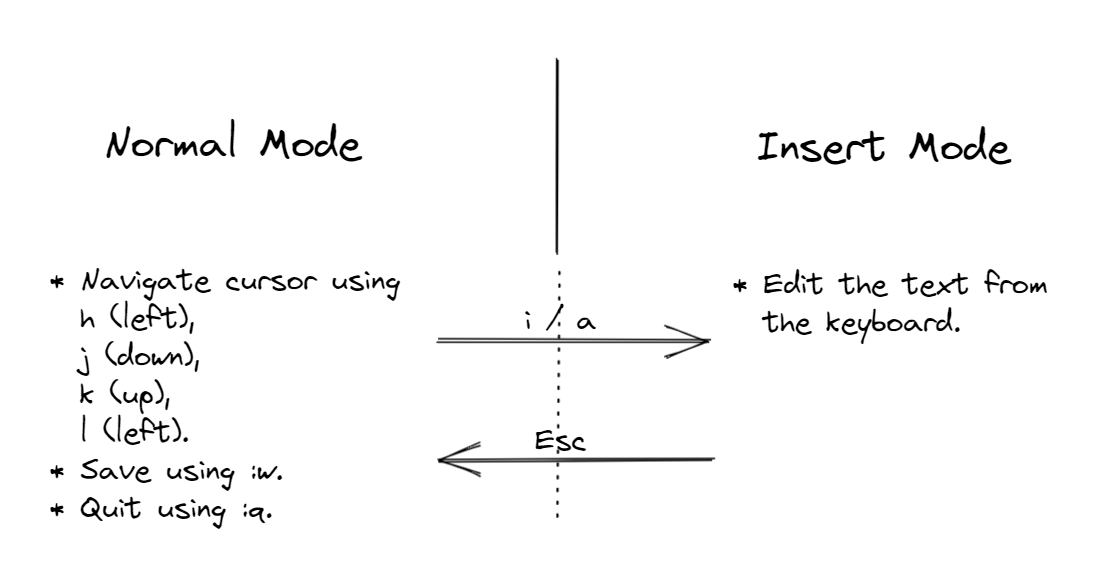
\includegraphics[width=250pt]{chapters/chapter4/figures/vimbasicmodeswitching.png}
\caption{Mode switching between normal mode and insert mode, and basic functions associated with the modes.} \label{ch4fig:vimbasicmodeswitching}
\end{figure}

\begin{figure}
\centering
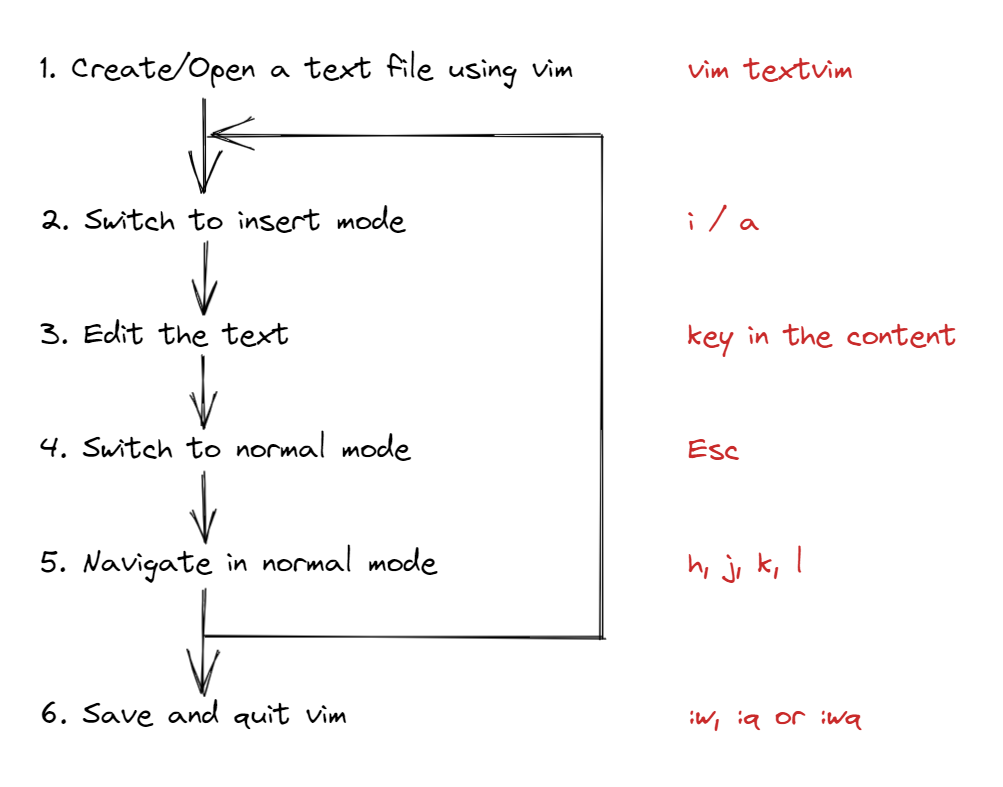
\includegraphics[width=250pt]{chapters/chapter4/figures/vimbasicoperationflowchart.png}
\caption{A flowchart for simple creating, editing and saving of a text file using \textit{Vim}.} \label{ch4fig:vimbasicoperationflowchart}
\end{figure}

\subsection{Configure Customizable User Profile}

With the basic operations introduced in Section \ref{ch4subsec:vimgeneralintro}, we are able to create and edit a text file as we want to, just like using any other text editor. Though at this point the advantages of using \textit{Vim} over other text editors are not obvious yet, the \textit{Vim} editor is finally useful now.

Before introducing more advanced features of \textit{Vim} for more convenient user experience, we can now customize user profile to suit our individual habit. Notice that the customization is completely optional and personal. This section only introduces the ideas and basic methods of such customization, such as re-mapping keys and create user-defined shortcuts. Everything introduced here are merely examples and it is completely up to the user how to design and implement his own profile.

In Linux, navigate to home directory. Create the following path and file \verb|~/.vim/vimrc| or \verb|~/.vimrc|. Open the \textit{vimrc} file as a blank file using \textit{Vim}. The individual user profile can be customized here.
\\
\\
\noindent \textbf{Mapping of Keys}
\\
\\
It is desirable to re-map some keys to speed up editing. For example, people may want to map \verb|jj| to \verb|Esc| in insert mode for more convenient mode switching to normal mode (consequent ``jj'' is rarely used in English). Other people may feel like mapping \verb|j|, \verb|k|, \verb|i| to \verb|h|, \verb|j|, \verb|k| respectively in normal and visual modes, making the navigation more intuitive. In that case, a different key needs to be mapped for \verb|i| since it is an important key for switching to insert mode.

It is possible re-map certain key (or keys combination) in selected modes. The following configuration in \textit{vimrc} file re-maps the aforementioned keys. 
\begin{verbatim}
inoremap jj <Esc>
noremap j h
noremap J H
noremap k j
noremap K J
noremap i k
noremap I K
noremap h i
noremap H I
\end{verbatim}
where \verb|inoremap| is used to map keys (combinations) in insert mode, and \verb|noremap| in normal and visual modes.

The upper case letter \verb|S| and lower case letter |s| in control mode are originally used to delete and substitute texts. They may be not so important in practice as there functions are overlapped by another shortcut key \verb|c|, which is powerful in replacing characters and is more frequently used. We can re-map \verb|S| for saving the text, and disable \verb|s| to prevent mis-touching. Similarly, upper case letter \verb|Q| is mapped to quit \textit{Vim}.
\begin{verbatim}
noremap s <nop>
map S :w<CR>
map Q :q<CR>
\end{verbatim}
where \verb|<nop>| stands for ``no operation'' and \verb|CR| stands for the ``enter'' key on the keyboard. The keyword \verb|map| differs from \verb|noremap| in the sense that \verb|map| is for recursive mapping.
\\
\\
\noindent \textbf{Syntax Highlight, Color Scheme and Others}
\\
\\
By default \textit{Vim} displays white color contents on black background. Use the following command in \textit{vimrc} to enable syntax highlighting or change color scheme. Use \verb|:colorscheme| in normal mode in \textit{Vim} to check for available color schemes.
\begin{verbatim}
syntax on
colorscheme default
\end{verbatim}




\subsection{Commonly Used Operations in Normal Mode}



